\documentclass[aspectratio=169, 10pt]{beamer}
\usetheme{default}
\useinnertheme{rectangles}
\usepackage[T1]{fontenc}
\usepackage{lmodern}
\usepackage{pgfplots}
\pgfplotsset{compat=1.18}

% Main colours for the header band and box titles.
\definecolor{band}{HTML}{0B4F6C}
\definecolor{highlight}{HTML}{01BAEF}

\setbeamercolor{block title}{fg=white, bg=band}
\setbeamercolor{block body}{fg=black, bg=band!6}
\setbeamercolor{block title alerted}{fg=white, bg=highlight!80!black}
\setbeamercolor{block body alerted}{fg=black, bg=highlight!10}
\setbeamercolor{itemize item}{fg=band}
\setbeamerfont{block title}{size=\small, series=\bfseries}
\setbeamertemplate{navigation symbols}{}
\setbeamertemplate{blocks}[rounded]
\setbeamersize{text margin left=0.4cm, text margin right=0.4cm}

\begin{document}

\begin{frame}[plain, t]
  % Header band: edit the title, authors and affiliation.
  \begin{tikzpicture}[remember picture, overlay]
    \fill[band] (current page.north west) rectangle ([yshift=-1.55cm]current page.north east);
    \node[anchor=north west, text=white, font=\Large\bfseries] at ([xshift=0.4cm, yshift=-0.25cm]current page.north west)
      {Urban Trees Cool Streets by Up to 4\,\textdegree C};
    \node[anchor=north west, text=white!85!band, font=\footnotesize] at ([xshift=0.4cm, yshift=-0.95cm]current page.north west)
      {M. Haddad, L. Fontaine, R. Osei \quad Centre for Urban Climate, Example City};
    \node[anchor=north east, draw=white, text=white, font=\tiny, minimum width=1.6cm, minimum height=1cm]
      at ([xshift=-0.4cm, yshift=-0.25cm]current page.north east) {Logo placeholder};
  \end{tikzpicture}
  \vspace{1.45cm}

  \begin{columns}[T, onlytextwidth]
    \begin{column}{0.31\textwidth}
      \begin{block}{Question}
        How much does tree canopy lower street temperature on hot afternoons?
      \end{block}
      \begin{block}{Method}
        \begin{itemize}
          \item 120 street sensors, summer 2025
          \item Canopy cover from aerial survey
          \item Linear mixed model by district
        \end{itemize}
      \end{block}
    \end{column}

    \begin{column}{0.36\textwidth}
      \begin{block}{Result}
        \centering
        % Replace the coordinates with your own data.
        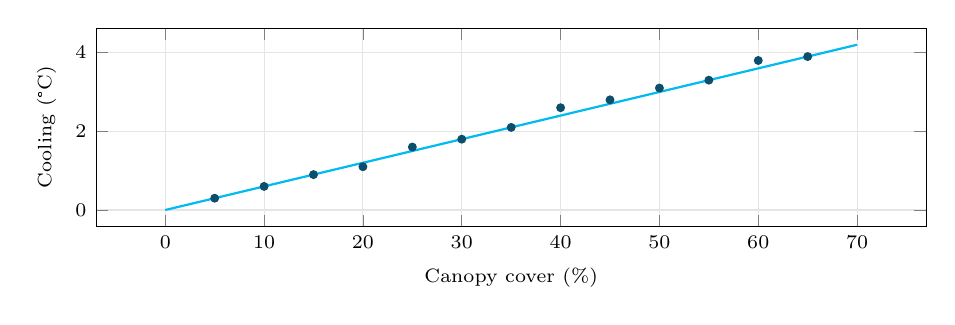
\begin{tikzpicture}
          \begin{axis}[width=\linewidth, height=4.1cm, xlabel={Canopy cover (\%)},
              ylabel={Cooling (\textdegree C)}, font=\scriptsize, grid=major, grid style={gray!20}]
            \addplot[only marks, mark size=1.4pt, band] coordinates {
              (5,0.3) (10,0.6) (15,0.9) (20,1.1) (25,1.6) (30,1.8) (35,2.1)
              (40,2.6) (45,2.8) (50,3.1) (55,3.3) (60,3.8) (65,3.9)};
            \addplot[thick, highlight, domain=0:70] {0.06*x};
          \end{axis}
        \end{tikzpicture}
      \end{block}
    \end{column}

    \begin{column}{0.29\textwidth}
      \begin{alertblock}{Key message}
        Every 10\% of canopy adds about 0.6\,\textdegree C of cooling.
      \end{alertblock}
      \begin{block}{Implications}
        \begin{itemize}
          \item Prioritise treeless streets
          \item Plan for shade, not just trees
        \end{itemize}
      \end{block}
      \begin{block}{Contact}
        \footnotesize m.haddad@example.org
      \end{block}
    \end{column}
  \end{columns}
\end{frame}

\end{document}
